\let\negmedspace\undefined
\let\negthickspace\undefined
\documentclass[journal,12pt,onecolumn]{IEEEtran}
\usepackage{cite}
\usepackage{amsmath,amssymb,amsfonts,amsthm}
\usepackage{algorithmic}
\usepackage{graphicx}
\usepackage{textcomp}
\usepackage{xcolor}
\usepackage{txfonts}
\usepackage{listings}
\usepackage{enumitem}
\usepackage{mathtools}
\usepackage{gensymb}
\usepackage{comment}
\usepackage[breaklinks=true]{hyperref}
\usepackage{tkz-euclide}
\usepackage{tikz}
\usetikzlibrary{calc, positioning, arrows.meta}
\usepackage{listings}
 % Commented out to prevent compilation errors if custom package is missing
%\def\inputGnumericTable{}
\usepackage[latin1]{inputenc}
\usepackage{color}
\usepackage{array}
\usepackage{longtable}
\usepackage{calc}
\usepackage{multirow}
\usepackage{hhline}
\usepackage{ifthen}
\usepackage{lscape}
\usepackage{tabularx}
\usepackage{array}
\usepackage{float}
\usepackage{caption}
\usepackage{multicol}
\usepackage{pgfplots}
\pgfplotsset{compat=1.18}

\newtheorem{theorem}{Theorem}[section]
\newtheorem{problem}{Problem}
\newtheorem{proposition}{Proposition}[section]
\newtheorem{lemma}{Lemma}[section]
\newtheorem{corollary}[theorem]{Corollary}
\newtheorem{example}{Example}[section]
\newtheorem{definition}[problem]{Definition}
\newcommand{\BEQA}{\begin{eqnarray}}
\newcommand{\EEQA}{\end{eqnarray}}
%\newcommand{\define}{\stackrel{\triangle}{=}}
\theoremstyle{remark}
%\newtheorem{rem}{Remark}


\title{Summary: GATE AE 2026 Paper}
\author{Arjun Iyengar \\ ee26btech11202 \\ IIT Hyderabad}
\date{August 2026}


\begin{document}

\maketitle

\section{PNC- Number of 3 digit numbers}

\noindent \textbf{Problem Statement:} \\ How many 3-digit numbers can be formed using three distinct single digit prime numbers?

\begin{enumerate}
    \item[(A)] $64$
    \item[(B)] $24$
    \item[(C)] $12$
    \item[(D)] $4$
\end{enumerate}
\subsection*{Step-by-Step Solution}

\noindent \textbf{Step 1:} There are 4 single digit prime numbers: 2,3,5 and 7. To make a three digit number, we choose 3 out of these and arrange them.\\ \\
  \textbf{Step 2:} Number of ways to choose three numbers = ${}^4C_3$ and number of way to arrange them = 3!\\ \\
  \textbf{Step 3:} By multiplication principle, total number of ways to achieve our requirement = ${}^4C_3 \times 3! = 4 \times 6 = 24$\\ \\

\section{Problems on Probability}
\subsection{Number of students in a class}

\noindent \textbf{Problem statement:}\\ In a group of students, 10 students like Mathematics, 12 students like English, 4 students like both Mathematics and English, and 6 students like neither Mathematics nor English. The number of students in the group is \underline{\hspace{1cm}}.

\begin{enumerate}
    \item[(A)] $18$
    \item[(B)] $20$
    \item[(C)] $24$
    \item[(D)] $32$
\end{enumerate}


\subsection*{Step-By-Step Solution (Probability-Based Method):}

 \textbf{Step 1:} Let $N$ be the total number of students in the group. 

\noindent If one student is chosen uniformly at random from the group, define:
\begin{itemize}
    \item $M$: The event that the student likes Mathematics.
    \item $E$: The event that the student likes English.
\end{itemize}

 \noindent\textbf{Step 2:} The respective probabilities are expressed as:
\begin{align*}
P(M) &= \frac{10}{N} \\[1ex]
P(E) &= \frac{12}{N} \\[1ex]
P(ME) &= \frac{4}{N} \quad \text{(student likes both)} \\[1ex]
P((M \cup E)') &= \frac{6}{N} \quad \text{(student likes neither)}
\end{align*}

\noindent\textbf{Step 3:} Since the total probability of the sample space is $1$:
\begin{align*}
P(M \cup E) + P((M \cup E)') = 1
\end{align*}

\noindent\textbf{Step 4:} Applying the Addition Theorem of Probability:
\begin{align*}
P(M) + P(E) - P(ME) + P((M \cup E)') = 1
\end{align*}

\noindent\textbf{Step 5:} Substitute the probabilities in terms of $N$:
\begin{align*}
\frac{10}{N} + \frac{12}{N} - \frac{4}{N} + \frac{6}{N} = 1
\end{align*}

\begin{align*}
\frac{10 + 12 - 4 + 6}{N} = 1
\end{align*}
\begin{align*}
\frac{24}{N} = 1 \implies N = 24
\end{align*}

\vspace{0.2cm}
\noindent \textbf{Correct Answer:} \textbf{(C) 24}




\subsection{Problem on manipulating probabilities}
\noindent \textbf{Problem statement:}\\
Consider two events $A$ and $B$ in a sample space $S$. We know the following data:
\begin{align*}
P(A), \quad P(B), \quad P(AB), \quad P((A \cup B)')
\end{align*}

\noindent Find the value of $P(AB')$ using the following formulae:
    \begin{align*}
    A + A' = 1, \quad AA' = 0
    \end{align*}
    \begin{align*}P(1) = 1, \quad P(0) = 0 \implies P(A + A') = 1, \quad P(AA') = 0
    \end{align*}
    \begin{align*}
    P(A + A') = P(A) + P(A')
    \end{align*}

\subsection*{Step-By-Step Solution:}
\noindent \textbf{Step 1: Express event $A$ using the Identity $B + B' = 1$} \\
Using the given identity that for any event $B$, $B + B' = 1$:
\begin{align*}
A = A \cdot 1 = A(B + B')
\end{align*}
Applying the distributive law:
\begin{align*}
A = AB + AB'
\end{align*}

\vspace{0.3cm}
\noindent \textbf{Step 2: Verify that $AB$ and $AB'$ are Mutually Exclusive} \\
To apply the additive property of probability, we check the intersection of $AB$ and $AB'$:
\begin{align*}
(AB)(AB') = A \cdot A \cdot B \cdot B' = A \cdot (BB')
\end{align*}
Since $BB' = 0$:
\begin{align*}
(AB)(AB') = A \cdot 0 = 0
\end{align*}
Thus, the events $AB$ and $AB'$ are mutually exclusive.

\vspace{0.3cm}
\noindent \textbf{Step 3: Apply the Probability Addition Rule} \\
Since $A = AB + AB'$ and $(AB)(AB') = 0$, we apply $P(X + Y) = P(X) + P(Y)$:
\begin{align*}
P(A) = P(AB + AB') = P(AB) + P(AB')
\end{align*}

\vspace{0.3cm}
\noindent \textbf{Step 4: Solve for $P(AB')$} \\
Rearranging the equation from Step 3 to isolate $P(AB')$:
\begin{align*}
{P(AB') = P(A) - P(AB)}
\end{align*}

\vspace{0.3cm}
\noindent \textbf{Final Answer:}
\begin{align*}
\mathbf{P(AB') = P(A) - P(AB)}     
\end{align*}

\section{Touching square and circles}

\enlargethispage{\baselineskip}
\noindent \textbf{Problem Statement:} \\ Given a square of side $s=4cm$ and two circles, onw with known radius $r_1=1cm$ and another with unkown radius $r_2$, such that both of them touch each other externally and also the square, find the value of $r_2$. Also describe how the figure in the problem can be drawn.
\begin{center}
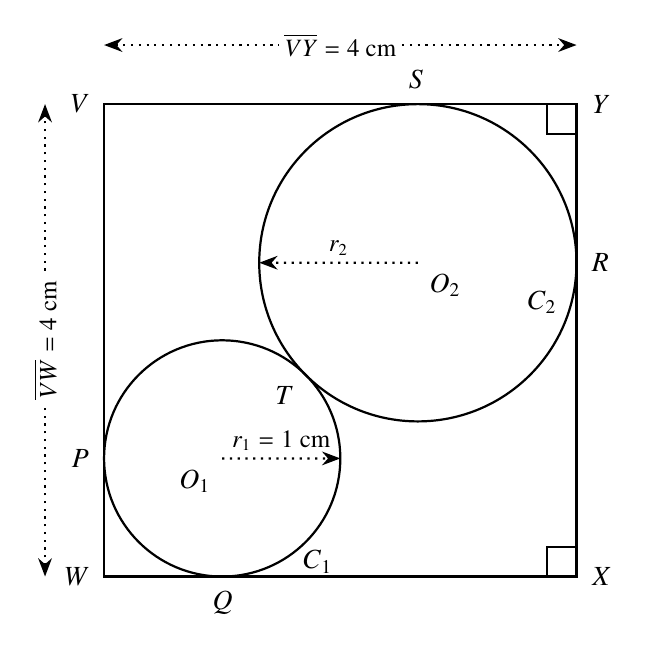
\begin{tikzpicture}[scale=1.5, >=Stealth]
    \pgfmathsetmacro{\side}{4.0}
    \pgfmathsetmacro{\rone}{1.0}
    \pgfmathsetmacro{\rtwo}{7 - 4*sqrt(2)}

    \coordinate (W) at (0, 0);
    \coordinate (X) at (\side, 0);
    \coordinate (Y) at (\side, \side);
    \coordinate (V) at (0, \side);

    \draw[thick] (W) -- (X) -- (Y) -- (V) -- cycle;

    \draw[thick] (\side-0.25, \side) -- (\side-0.25, \side-0.25) -- (\side, \side-0.25);
    \draw[thick] (\side-0.25, 0) -- (\side-0.25, 0.25) -- (\side, 0.25);

    \coordinate (O1) at (\rone, \rone);
    \coordinate (O2) at (\side-\rtwo, \side-\rtwo);

    \coordinate (P) at (0, \rone);
    \coordinate (Q) at (\rone, 0);
    \coordinate (S) at (\side-\rtwo, \side);
    \coordinate (R) at (\side, \side-\rtwo);

    \pgfmathsetmacro{\Tx}{\rone + \rone*cos(45)}
    \pgfmathsetmacro{\Ty}{\rone + \rone*sin(45)}
    \coordinate (T) at (\Tx, \Ty);

    \draw[thick] (O1) circle (\rone);
    \draw[thick] (O2) circle (\rtwo);

    \draw[dotted, thick, ->] (O1) -- (2*\rone, \rone) 
        node[midway, above=-1pt] {\small $r_1 = 1\text{ cm}$};

    \draw[dotted, thick, ->] (O2) -- (\side-2*\rtwo, \side-\rtwo) 
        node[midway, above=-1pt] {\small $r_2$};

    \node[left=2pt] at (V) {$V$};
    \node[left=2pt] at (W) {$W$};
    \node[right=2pt] at (X) {$X$};
    \node[right=2pt] at (Y) {$Y$};

    \node[left=2pt] at (P) {$P$};
    \node[below=2pt] at (Q) {$Q$};
    \node[above=2pt] at (S) {$S$};
    \node[right=2pt] at (R) {$R$};
    \node[below left=1pt] at (T) {$T$};

    \node[below left=1pt] at (O1) {$O_1$};
    \node[below right=1pt] at (O2) {$O_2$};

    \node[below right] at (1.6, 0.3) {$C_1$};
    \node[below right] at (\side-0.5, \side-1.5) {$C_2$};

    \draw[dotted, thick, <->] (0, \side+0.5) -- (\side, \side+0.5) 
        node[midway, fill=white, inner sep=2pt] {\small $\overline{VY} = 4\text{ cm}$};

    \draw[dotted, thick, <->] (-0.5, 0) -- (-0.5, \side) 
        node[midway, fill=white, inner sep=2pt, rotate=90] {\small $\overline{VW} = 4\text{ cm}$};

\end{tikzpicture}
\end{center}
\subsection*{Step-by-Step Solution:}

    \noindent \textbf{Step 1}: Let the side of the square be $s$, radius of the first circle be $r_1$ and that of the unknown circle be $r_2$.\\ \\
    \textbf{Step 2:} Clearly from figure:
     \begin{align*}
      \overline{WO_1}+ \overline{O_1T}+ \overline{TO_2} +\overline{O_2Y}= \sqrt{2}s 
     \end{align*}
     \textbf{Step 3:} We know that:
     \begin{align*}
     \overline{WO_1} = \sqrt{2}r_1,    \overline{O_1T} = r_1, \overline{TO_2} = r_2 , \overline{O_2W} = \sqrt{2}r_2. 
     \end{align*}
     \textbf{Step 4:} Substituting this in our result from point 2, we get $r_2 = \frac{\sqrt{2}s - (\sqrt{2} + 1)r_1}{\sqrt{2} + 1}$. \\ \\
     \textbf{Step 5:} Substituting the values of $s$ and $r_1$, we get $r_2$=$7-4\sqrt{2}cm$ \\ \\
     \textbf{Step 6:} Now to draw the figure, we assign coordinates to vertices of the square( say (0,0), ($s$,0), ($s$,$s$) and ($s$,0), the centre of the first circle ($r_1$,$r_1$) and the centre of the third circle($s-r_2$,$s-r_2$) to get the plot.\\ \\
     
     
     




\section{Problem on line integrals}
\noindent \textbf{Problem statement:}\\ Consider the contour $C$ shown in the figure below. For the vector $\vec{F} = (x + 2y)\hat{e}_x + (2x + 4y)\hat{e}_y$, the integral $\oint_{C} \vec{F} \cdot d\vec{l} = \underline{\hspace{2cm}}$.

\vspace{0.5em}
\noindent Here $d\vec{l}$ represents an infinitesimal length along the contour $C$.\\ 
\begin{center}
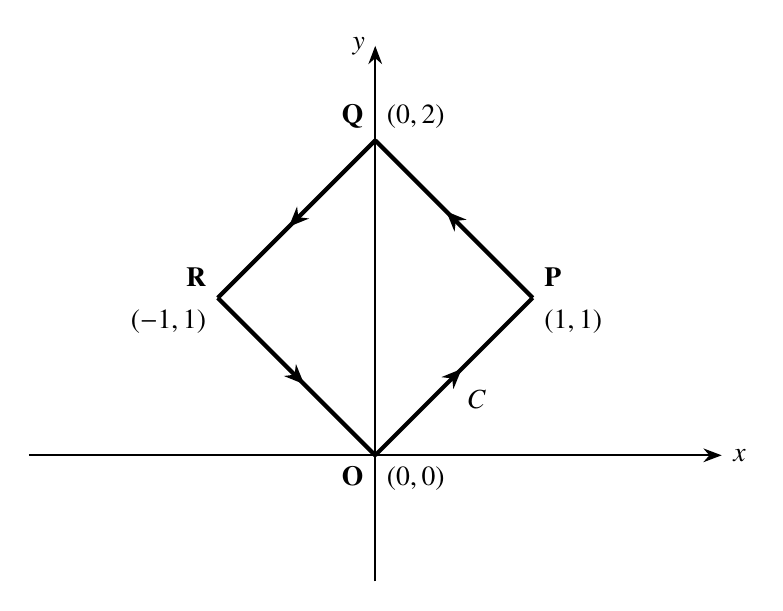
\begin{tikzpicture}[scale=2, >=Stealth]
    \tikzset{
        segment arrow/.style={
            postaction={
                decorate,
                decoration={
                    markings,
                    mark=at position 0.55 with {\arrow[scale=1.2]{Stealth[length=6pt, width=5pt]}}
                }
            }
        }
    }

    \draw[thick, ->] (-2.2, 0) -- (2.2, 0) node[right] {$x$};
    \draw[thick, ->] (0, -0.8) -- (0, 2.6) node[left] {$y$};

    \coordinate (O) at (0, 0);
    \coordinate (P) at (1, 1);
    \coordinate (Q) at (0, 2);
    \coordinate (R) at (-1, 1);

    \draw[line width=1.5pt, segment arrow] (O) -- (P);
    \draw[line width=1.5pt, segment arrow] (P) -- (Q);
    \draw[line width=1.5pt, segment arrow] (Q) -- (R);
    \draw[line width=1.5pt, segment arrow] (R) -- (O);

    \node[below right=2pt] at (0.5, 0.5) {$C$};

    \node[below left=1pt] at (O) {$\mathbf{O}$};
    \node[below right=1pt] at (O) {$(0,0)$};

    \node[above right=1pt] at (P) {$\mathbf{P}$};
    \node[below right=1pt] at (P) {$(1,1)$};

    \node[above left=1pt] at (Q) {$\mathbf{Q}$};
    \node[above right=1pt] at (Q) {$(0,2)$};

    \node[above left=1pt] at (R) {$\mathbf{R}$};
    \node[below left=1pt] at (R) {$(-1,1)$};

\end{tikzpicture}
\end{center}

\noindent We can break the closed path $C$ into its four straight line paths: $O \to P \to Q \to R \to O$.
\noindent The general line integral expression to evaluate along any path is:
\begin{align*}
\mathbf{I} = \int (x + 2y)\,dx + (2x + 4y)\,dy
\end{align*}
\subsection*{Step-by-Step Solution:}

\subsection*{1. Path $O(0,0) \to P(1,1)$}
\begin{itemize}
    \item \textbf{Equation of line:} $y = x \implies dy = dx$
    \item \textbf{Limits:} $x$ goes from $0$ to $1$
\end{itemize}
\begin{align*}
\mathbf{I_1} = \int_0^1 (x + 2x)\,dx + (2x + 4x)\,dx = \int_0^1 9x\,dx = \left[ \frac{9x^2}{2} \right]_0^1 = \frac{9}{2}
\end{align*}

\subsection*{2. Path $P(1,1) \to Q(0,2)$}
\begin{itemize}
    \item \textbf{Equation of line:} $y = 2 - x \implies dy = -dx$
    \item \textbf{Limits:} $x$ goes from $1$ to $0$
\end{itemize}
\begin{align*}
\mathbf{I_2} = \int_1^0 (x + 2(2-x))\,dx + (2x + 4(2-x))(-dx)
\end{align*}
\begin{align*}
\mathbf{I_2} = \int_1^0 \left[ (4-x) - (8-2x) \right]\,dx = \int_1^0 (x-4)\,dx = \left[ \frac{x^2}{2} - 4x \right]_1^0 = \frac{7}{2}
\end{align*}

\subsection*{3. Path $Q(0,2) \to R(-1,1)$}
\begin{itemize}
    \item \textbf{Equation of line:} $y = x + 2 \implies dy = dx$
    \item \textbf{Limits:} $x$ goes from $0$ to $-1$
\end{itemize}
\begin{align*}
\mathbf{I_3} = \int_0^{-1} (x + 2(x+2))\,dx + (2x + 4(x+2))\,dx = \int_0^{-1} (9x + 12)\,dx
\end{align*}
\begin{align*}
\mathbf{I_3} = \left[ \frac{9x^2}{2} + 12x \right]_0^{-1} = \left(\frac{9}{2} - 12\right) - 0 = -\frac{15}{2}
\end{align*}

\subsection*{4. Path $R(-1,1) \to O(0,0)$}
\begin{itemize}
    \item \textbf{Equation of line:} $y = -x \implies dy = -dx$
    \item \textbf{Limits:} $x$ goes from $-1$ to $0$
\end{itemize}
\begin{align*}
\mathbf{I_4} = \int_{-1}^0 (x + 2(-x))\,dx + (2x + 4(-x))(-dx) = \int_{-1}^0 x\,dx
\end{align*}
\begin{align*}
\mathbf{I_4} = \left[ \frac{x^2}{2} \right]_{-1}^0 = 0 - \frac{1}{2} = -\frac{1}{2}
\end{align*}

\subsection*{Total Line Integral}
Summing the integrals across all four line segments:
\begin{align*}
\mathbf{I = I_1 + I_2 + I_3 + I_4}
\end{align*}
\begin{align*}
\mathbf{I} = \frac{9}{2} + \frac{7}{2} - \frac{15}{2} - \frac{1}{2} = \frac{16 - 16}{2} = 0
\end{align*}

\section{The Fourier transform}
\subsection{Problem on evaluating an integral and verifying}
\noindent \textbf{Problem Statement:} \\
Consider $x(t)$ to be defined as
\begin{align*}
{x(t)} = 
\begin{cases} 
1, & t \in (-1, 1) \\ 
0, & \text{otherwise} 
\end{cases}
\end{align*}

\noindent Consider
\begin{align*}
\mathbf{c_k} = f_0 \int_{-\frac{1}{2f_0}}^{\frac{1}{2f_0}} x(t) e^{-j 2\pi k f_0 t} \, dt
\end{align*}

\noindent Taking frequency $f_0 = \frac{1}{4}$, solve for $c_k$.
\subsection*{Step-by-Step Solution:}
\noindent \textbf{Step 1: Substitute $f_0 = \frac{1}{4}$ into the Integral Expression} \\
Given $f_0 = \frac{1}{4}$, the upper and lower limits of integration become:
\begin{align*}
\frac{1}{2f_0} = \frac{1}{2(1/4)} = 2, \quad -\frac{1}{2f_0} = -2
\end{align*}
Substituting $f_0 = \frac{1}{4}$ into $c_k$:
\begin{align*}
\mathbf{c_k} = \frac{1}{4} \int_{-2}^{2} x(t) e^{-j \left(\frac{\pi k t}{2}\right)} \, dt
\end{align*}

\vspace{0.3cm}
\noindent \textbf{Step 2: Substitute $x(t)$ into the Integral} \\
Since $x(t) = 1$ for $t \in (-1, 1)$ and $0$ otherwise, the limits of integration reduce to $[-1, 1]$:
\begin{align*}
\mathbf{c_k} = \frac{1}{4} \int_{-1}^{1} e^{-j \left(\frac{\pi k t}{2}\right)} \, dt
\end{align*}

\vspace{0.3cm}
\noindent \textbf{Step 3: Expand the Exponential using Euler's Formula} \\
Using Euler's formula, $e^{j\theta} = \cos\theta + j\sin\theta$, we write:
\begin{align*}
\mathbf{c_k} = \frac{1}{4} \int_{-1}^{1} \left[ \cos\left(\frac{\pi k t}{2}\right) - j \sin\left(\frac{\pi k t}{2}\right) \right] \, dt
\end{align*}

\vspace{0.3cm}
\noindent \textbf{Step 4: Integrate the Trigonometric Terms} \\
Performing the integration with respect to $t$:
\begin{align*}
\mathbf{c_k} = \frac{1}{2\pi k} \left[ \left. \sin\left(\frac{\pi k t}{2}\right) \right|_{-1}^{1} + \left. j \cos\left(\frac{\pi k t}{2}\right) \right|_{-1}^{1} \right]
\end{align*}

\vspace{0.3cm}
\noindent \textbf{Step 5: Evaluate at the Limits $t = 1$ and $t = -1$} \\
Substitute the upper and lower limits:
\begin{align*}
\mathbf{c_k} = \frac{1}{2\pi k} \left[ \sin\left(\frac{\pi k}{2}\right) - \sin\left(-\frac{\pi k}{2}\right) + j \left( \cos\left(\frac{\pi k}{2}\right) - \cos\left(-\frac{\pi k}{2}\right) \right) \right]
\end{align*}
Since $\sin(-x) = -\sin(x)$ and $\cos(-x) = \cos(x)$:
\begin{align*}
\mathbf{c_k} = \frac{1}{2\pi k} \left[ \sin\left(\frac{\pi k}{2}\right) + \sin\left(\frac{\pi k}{2}\right) + j(0) \right]
\end{align*}

\vspace{0.3cm}
\noindent \textbf{Step 6: Simplify to Obtain the Final Result} \\
Combining like terms:
\begin{align*}
\mathbf{c_k} = \frac{1}{2\pi k} \left[ 2 \sin\left(\frac{\pi k}{2}\right) \right]
\end{align*}
\begin{align*}
\mathbf{c_k = \frac{\sin\left(\frac{\pi k}{2}\right)}{\pi k}}
\end{align*}

\subsection{The Gibbs Phenomenon}
\noindent \textbf{Problem Statement:} \\The Fourier series representation of a square wave is shown in the figure below. The fluctuations seen near $x = \pm 1$ are named after which one of the following scientists?
\begin{center}
    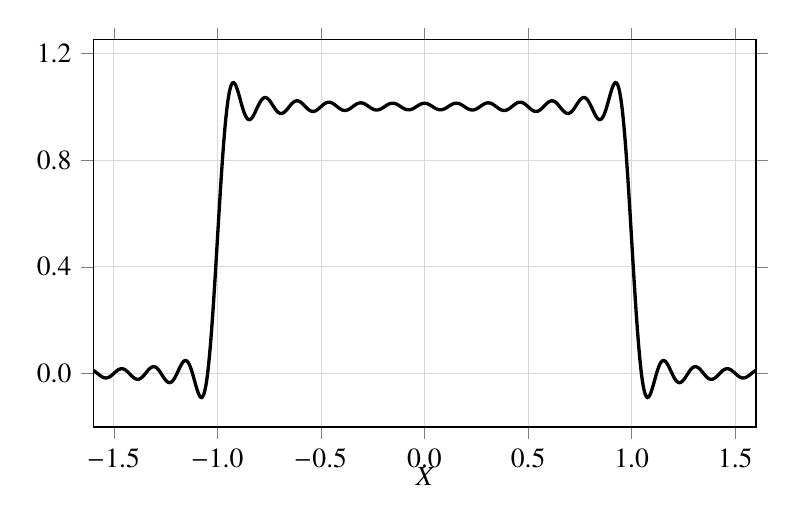
\begin{tikzpicture}
\begin{axis}[
    width=10cm,
    height=6.5cm,
    xmin=-1.6, xmax=1.6,
    ymin=-0.2, ymax=1.25,
    xtick={-1.5, -1.0, -0.5, 0.0, 0.5, 1.0, 1.5},
    ytick={0.0, 0.4, 0.8, 1.2},
    xticklabel style={/pgf/number format/.cd, fixed, fixed zerofill, precision=1},
    yticklabel style={/pgf/number format/.cd, fixed, fixed zerofill, precision=1},
    grid=major,
    grid style={line width=0.3pt, draw=gray!30},
    xlabel={$X$},
    xlabel style={at={(axis description cs:0.5,-0.08)}, anchor=north},
    trig format=rad,
    tick align=outside,
    axis line style={black}
]

\addplot[
    domain=-1.6:1.6,
    samples=600,
    very thick,
    black
]
{0.5 + (2/pi)*(
    cos(pi*x/2) 
    - (1/3)*cos(3*pi*x/2) 
    + (1/5)*cos(5*pi*x/2) 
    - (1/7)*cos(7*pi*x/2) 
    + (1/9)*cos(9*pi*x/2) 
    - (1/11)*cos(11*pi*x/2) 
    + (1/13)*cos(13*pi*x/2) 
    - (1/15)*cos(15*pi*x/2) 
    + (1/17)*cos(17*pi*x/2) 
    - (1/19)*cos(19*pi*x/2) 
    + (1/21)*cos(21*pi*x/2) 
    - (1/23)*cos(23*pi*x/2) 
    + (1/25)*cos(25*pi*x/2)
)};

\end{axis}
\end{tikzpicture}
\end{center}

\vspace{0.5em}
\begin{enumerate}
    \item[(A)] Cauchy
    \item[(B)] Fourier
    \item[(C)] Gibbs
    \item[(D)] Laplace
\end{enumerate}
\subsection*{Solution:}
\noindent Gibbs phenomenon is the overshoot and high-frequency oscillation ("ringing") that occurs when approximating a function with jump discontinuities using a finite (truncated) Fourier series.Even as the number of terms $N$ approaches infinity, the overshoot near the jump discontinuity does not vanish; instead, it narrows in width while maintaining a fixed percentage height relative to the size of the jump.\\ \\
\noindent \textbf{Reason:} When approximating a step function or square wave, Fourier series synthesize the shape using smooth, continuous sinusoids ($\sin$ and $\cos$). Because continuous functions cannot instantaneously step from one value to another, the Fourier series overcompensates near the vertical edge.\\ \\
\noindent \textbf{Final Answer: (C) Gibbs }\\ 

\newpage

\section{Solving for value of determinant}

\noindent \textbf{Problem Statement:} \\
An $n \times n$ square matrix $\mathbf{A}$ satisfies $\mathbf{A^T} = \mathbf{A^{-1}}$. The determinant of this matrix may take which of the following value(s)?

\subsection*{Step-by-Step Solution:}

\noindent \textbf{Step 1:}  We are given that matrix $A$ satisfies:
\begin{align*}
\mathbf{A^T = A^{-1}}
\end{align*}

\noindent \textbf{Step 2:} 
Taking the determinant of both sides of the given matrix equation:
\begin{align*}
\det(\mathbf{A^T}) = \det(\mathbf{A^{-1}})
\end{align*}

\noindent \textbf{Step 3:}
Recall the fundamental properties of matrix determinants:
\begin{itemize}
        \item Transpose property: $\det(\mathbf{A^T}) = \det(\mathbf{A})$
        \item Inverse property: $\det(\mathbf{A^{-1}}) = \frac{1}{\det(\mathbf{A)}}$
    \end{itemize} 

\noindent \textbf{Step 4:} 
Replacing both sides using the above properties gives:
\begin{align*}
\det(\mathbf{A}) = \frac{1}{\det(\mathbf{A})}
\end{align*}

\noindent  \textbf{Step 5:}
Multiplying both sides by $\det(\mathbf{A})$:
 \begin{align*}
(\det(\mathbf{A}))^2 = 1 \implies \det(\mathbf{A}) = \pm 1
\end{align*} 


\noindent \textbf{Correct Options:} \textbf{(A)} $+1$ and \textbf{(B)} $-1$

\section*{Proof that $\det(\mathbf{A^T}) = \det(\mathbf{A})$}

\noindent When expanding $\det(\mathbf{A})$ along \textbf{Row 1}, you select entries across the top row and compute the determinants of their remaining submatrices.

\vspace{0.3cm}

\noindent When expanding $\det(\mathbf{A^T})$ down \textbf{Column 1}, those exact same entries now sit vertically in the first column, and their corresponding submatrices are simply transposed!

\vspace{0.8cm}

\subsection*{Visual Matrix Comparison}

\noindent
\textbf{Matrix $\mathbf{A}$ (Expand along Row 1):}
\begin{align*}
\det(\mathbf{A}) = 
\begin{vmatrix}
\mathbf{a_{11}} & \mathbf{a_{12}} & \mathbf{a_{13}} \\
a_{21} & a_{22} & a_{23} \\
a_{31} & a_{32} & a_{33}
\end{vmatrix}
\end{align*}

\noindent
\textbf{Matrix $\mathbf{A^T}$ (Expand down Column 1):}
\begin{align*}
\det(\mathbf{A^T}) = 
\begin{vmatrix}
\mathbf{a_{11}} & a_{21} & a_{31} \\
\mathbf{a_{12}} & a_{22} & a_{32} \\
\mathbf{a_{13}} & a_{23} & a_{33}
\end{vmatrix}
\end{align*}

\vspace{0.5cm}

\subsection*{Submatrix Comparison for Entry $a_{12}$}

When selecting $a_{12}$:
\begin{itemize}
    \item In $\mathbf{A}$ (Row 1, Column 2 deletion):
    \begin{align*}
    \mathbf{M_{12}} = \begin{bmatrix} a_{21} & a_{23} \\ a_{31} & a_{33} \end{bmatrix}
    \end{align*}

    \item In $\mathbf{A^T}$ (Row 2, Column 1 deletion):
    \begin{align*}
    \mathbf{N_{21}} = \begin{bmatrix} a_{21} & a_{31} \\ a_{23} & a_{33} \end{bmatrix}
    \end{align*}
\end{itemize}

\noindent Notice that $\mathbf{N_{21}} = (\mathbf{M_{12})^T}$. Since $\det(\mathbf{M_{12}}) = \det((\mathbf{M_{12}})^T)$, every term in the expansion of $\det(\mathbf{A})$ is identically equal to the corresponding term in $\det(\mathbf{A^T})$.
\newpage
\section{Problem on rank of a matrix and echeleon form}

\noindent \textbf{Problem Statement:} \\
If a matrix can be written as $\mathbf{A} = \mathbf{uv^T}$, where both $u$ and $v$ are $n$-dimensional real-valued non-zero column vectors, then the rank of the matrix $\mathbf{A}$ is \underline{\hspace{1cm}}.

\subsection*{Step-by-Step solution:}


    \noindent \textbf{Step 1:}
    The matrix $\mathbf{A}$ is formed by taking the outer product of two $n \times 1$ non-zero column vectors $\mathbf{u}$ and $\mathbf{v}$:
    \begin{align*}
    \mathbf{A = uv^T}
    \end{align*}
    Writing $\mathbf{u}$ and $\mathbf{v^T}$ explicitly:
    \begin{align*}
    \mathbf{u}= \begin{bmatrix} u_1 \\ u_2 \\ \vdots \\ u_n \end{bmatrix}, \quad
    \mathbf{v^T} = \begin{bmatrix} v_1 & v_2 & \dots & v_n \end{bmatrix}
    \end{align*}

    \noindent \textbf{Step 2:}
    Multiplying $\mathbf{u}$ and $\mathbf{v^T}$ gives the $n \times n$ matrix $\mathbf{A}$:
    \begin{align*}
    \mathbf{A} = \begin{bmatrix} 
    u_1 v_1 & u_1 v_2 & \dots & u_1 v_n \\ 
    u_2 v_1 & u_2 v_2 & \dots & u_2 v_n \\ 
    \vdots & \vdots & \ddots & \vdots \\ 
    u_n v_1 & u_n v_2 & \dots & u_n v_n 
    \end{bmatrix}
    \end{align*}

    \noindent \textbf{Step 3:}
    Notice that each column of $\mathbf{A}$ can be written as a scalar multiple of vector $\mathbf{u}$:
    \begin{itemize}
        \item 1st column: $v_1 \mathbf{u}$
        \item 2nd column: $v_2 \mathbf{u}$
        \item $j^{\text{th}}$ column: $v_j \mathbf{u}$
    \end{itemize}
    

    \noindent \textbf{Step 4:}
    \begin{itemize}
        \item The rank of a matrix is equal to the number of non zero rows in its echeleon form.
        \item When we reduce the above matrix into the echeleon form, we notice that each row is a multiple of another as shown above.
        \item Therefore, when we apply elementary row transformations by multiplying the rows with the necessary constants and subtracting, all rows but one become non zero.
        \item Hence, the rank of the matrix becomes  $1$.
    \end{itemize}




\noindent \textbf{Final Answer:} \textbf{1}


\section{Trajectory of satellite}

\noindent \textbf{Problem Statement:} Given the velocity and position vectors of a satellite along with its gravitational parameter $\mu=GM$, determine the trajectory of the satellite. \\ 
\textbf{Given Data:}
\begin{itemize}
    \item Position vector: 
    \begin{align*}
    \vec{r} = 8000\hat{p} + 9000\hat{q} \text{ km}
    \end{align*}
    \item Velocity vector:
    \begin{align*}
    \vec{v} = -6\hat{p} + 6\hat{q} \text{ km/s}
    \end{align*}
    \item Gravitational parameter: 
    \begin{align*}
    \mu = 398600 \text{ km}^3/\text{s}^2
    \end{align*}
\end{itemize}
\subsection*{Step-by-Step Solution:}

\noindent \textbf{Step 1: Calculate Magnitudes $r$ and $v^2$}\\
The magnitude of the position vector $r$ is:
\begin{align*}
r = |\vec{r}| = \sqrt{8000^2 + 9000^2} = \sqrt{64 \times 10^6 + 81 \times 10^6} = \sqrt{145 \times 10^6} \approx 12041.59 \text{ km}
\end{align*}

\noindent The square of the velocity magnitude $v^2$ is:
\begin{align*}
v^2 = |\vec{v}|^2 = (-6)^2 + (6)^2 = 36 + 36 = 72 \text{ (km/s)}^2
\end{align*}

\noindent \textbf{Step 2: Calculate Specific Mechanical Energy ($E$)}\\

\noindent The specific mechanical energy (energy per unit mass) is given by:
\noindent
\begin{align*}
E = \text{Kinetic Energy per unit mass} + \text{Potential Energy per unit mass}
\end{align*}
\begin{align*}
E = \frac{1}{2}v^2 - \frac{\mu}{r}
\end{align*}

\noindent Substituting the calculated values:
\begin{align*}
E &= \frac{72}{2} - \frac{398600}{12041.59} \\ \\
&= 36 - 33.102 \\ 
&= +2.898 \text{ km}^2/\text{s}^2
\end{align*}

\noindent \textbf{Step 3: Determine Trajectory Type}\\

The trajectory of an orbiting body is determined by the sign of its specific mechanical energy $E$:
\begin{itemize}
    \item $E < 0 \implies \text{Elliptic / Circular orbit (Bound)}$
    \item $E = 0 \implies \text{Parabolic trajectory (Unbound)}$
    \item $E > 0 \implies \text{Hyperbolic trajectory (Unbound)}$
\end{itemize}

Since $E = +2.898 > 0$, the satellite follows a \textbf{Hyperbolic trajectory}.

\vspace{0.3cm}
\noindent \textbf{Correct Answer:} \textbf{(B) Hyperbola}
\newpage

\section{Problem on eigenvectors and eigenvalues}

\noindent \textbf{Problem Statement:} For the matrix $A = \begin{bmatrix} a & b \\ c & d \end{bmatrix}$, if the relation $a + b = c + d$ holds and $a, b, c, d \neq 0$, then which one of the following statements about $A$ is FALSE?

\begin{enumerate}
    \item[(A)] $\begin{bmatrix} 1 \\ 1 \end{bmatrix}$ is an eigenvector
    \item[(B)] $\lambda = a + b$ is an eigenvalue
    \item[(C)] $\lambda = d - b$ is an eigenvalue
    \item[(D)] $\lambda = d + b$ is an eigenvalue
\end{enumerate}
\subsection*{Step-by-Step Solution}
\noindent {\textbf{Step 1: Check Eigenvector and First Eigenvalue}}

\noindent Given that $a + b = c + d = k$:
\begin{align*}
\begin{pmatrix} a & b \end{pmatrix} \begin{pmatrix} 1 \\ 1 \end{pmatrix} &= k = \begin{pmatrix} c & d \end{pmatrix} \begin{pmatrix} 1 \\ 1 \end{pmatrix} \\[1ex]
\implies \begin{pmatrix} a & b \\ c & d \end{pmatrix} \begin{pmatrix} 1 \\ 1 \end{pmatrix} &= \begin{pmatrix} k \\ k \end{pmatrix} \\[1ex]
\implies \begin{pmatrix} a & b \\ c & d \end{pmatrix} \begin{pmatrix} 1 \\ 1 \end{pmatrix} &= k \begin{pmatrix} 1 \\ 1 \end{pmatrix}
\end{align*}

\noindent $\therefore \begin{pmatrix} 1 \\ 1 \end{pmatrix}$ is an eigenvector and $k = a + b$ is an eigenvalue.

\vspace{0.5cm}

\noindent {\textbf{Step 2: Find the Second Eigenvalue}}

\noindent From the given relation $a + b = c + d$:
\begin{align*}
a - c = d - b = -(b - d) = k'
\end{align*}

\noindent Evaluating the matrix-vector multiplication:
\begin{align*}
\begin{pmatrix} a & b \\ c & d \end{pmatrix} \begin{pmatrix} 1 \\ -1 \end{pmatrix} &= \begin{pmatrix} a - b \\ c - d \end{pmatrix} = \begin{pmatrix} k' \\ -k' \end{pmatrix} = k' \begin{pmatrix} 1 \\ -1 \end{pmatrix}
\end{align*}

\noindent $\therefore \begin{pmatrix} 1 \\ -1 \end{pmatrix}$ is an eigenvector and $d - b$ is the $2^{\text{nd}}$ eigenvalue.

\vspace{0.5cm}

\noindent \textbf{Conclusion:}
\begin{itemize}
    \item Statement (A) is \textbf{TRUE}: $\begin{bmatrix} 1 \\ 1 \end{bmatrix}$ is an eigenvector.
    \item Statement (B) is \textbf{TRUE}: $\lambda = a + b$ is an eigenvalue.
    \item Statement (C) is \textbf{TRUE}: $\lambda = d - b$ is an eigenvalue.
    \item Statement (D) is \textbf{FALSE}: $\lambda = d + b$ is not an eigenvalue.
\end{itemize}

\noindent \textbf{Correct Answer:} \textbf{(D)}
\newpage

\newpage

\section{Differential equation using laplace transform}

\noindent \textbf{Problem Statement:} \\
Consider the differential equation:
\begin{align*}
\frac{d^2 y}{dx^2} + 2\frac{dy}{dx} + y = 0
\end{align*}
with initial conditions $\left.y\right|_{x=0} = 0$ and $\left.\frac{dy}{dx}\right|_{x=0} = 1$. Find the value of the slope $\frac{dy}{dx}$ at $x = \ln(2)$ rounded off to three decimal places.\\ \\
\subsection*{Step-by-Step Solution}

    \noindent \textbf{Step 1: Apply Laplace Transform}\\ \\
Let $Y(s) = \mathcal{L}\{y(x)\}$. Taking the Laplace transform on both sides:
\begin{align*}
\mathcal{L}\left\{\frac{d^2 y}{dx^2}\right\} + 2\mathcal{L}\left\{\frac{dy}{dx}\right\} + \mathcal{L}\{y\} = 0
\end{align*}

\noindent Using the standard operational properties:
\begin{align*}
\big[s^2 Y(s) - s y(0) - y'(0)\big] + 2\big[s Y(s) - y(0)\big] + Y(s) = 0
\end{align*}

\noindent Substituting the given initial conditions $y(0) = 0$ and $y'(0) = 1$:
\begin{align*}
(s^2 Y(s) - 1) + 2s Y(s) + Y(s) = 0
\end{align*}
\begin{align*}
(s^2 + 2s + 1) Y(s) = 1
\end{align*}
\begin{align*}
Y(s) = \frac{1}{(s+1)^2}
\end{align*}
\noindent \textbf{Step 2: Inverse Laplace Transform}\\ \\
\noindent Taking the inverse Laplace transform gives the solution $y(x)$:
\begin{align*}
y(x) = \mathcal{L}^{-1}\left\{\frac{1}{(s+1)^2}\right\} = x e^{-x}
\end{align*}
\noindent \textbf{Step 3: Calculate the Slope $\frac{dy}{dx}$} \\ \\
\noindent Differentiating $y(x)$ with respect to $x$:
\begin{align*}
\frac{dy}{dx} = \frac{d}{dx}\left(x e^{-x}\right) = (1 - x)e^{-x}
\end{align*}
\noindent \textbf{Step 4: Evaluate at $x = \ln(2)$} \\ \\
\noindent Substituting $x = \ln(2)$:
\begin{align*}
\left.\frac{dy}{dx}\right|_{x=\ln(2)} = \big(1 - \ln(2)\big) e^{-\ln(2)}
\end{align*}

\noindent Since $e^{-\ln(2)} = \frac{1}{2}$:
\begin{align*}
\left.\frac{dy}{dx}\right|_{x=\ln(2)} = \frac{1 - \ln(2)}{2} \approx \frac{1 - 0.693147}{2} = 0.153426
\end{align*}


\noindent Rounding off to three decimal places yields: \textbf{0.153}
\newpage

\section{Sub-Problems on laplace transform}
\subsection{Few proofs on laplace transform}
\noindent Consider a function $g(t)$ and let $G(s)$ be its Laplace transform. Show that:
\begin{enumerate}
    \item[(a)] Applying Laplace transform on $g'(t)$ gives $s G(s)$
    \item[(b)] Applying Laplace transform on $g''(t)$ gives $s^2 G(s)$
\end{enumerate}

\vspace{0.3cm}
\hrule
\vspace{0.5cm}

\noindent \textbf{Step-by-Step Solution \& Proof}

\noindent By definition, the Laplace transform of a function $f(t)$ is given by:
\begin{align*}
\mathcal{L}\{f(t)\} = \int_{0}^{\infty} e^{-st} f(t) \, dt = F(s)
\end{align*}

\noindent Given that $\mathcal{L}\{g(t)\} = G(s) = \int_{0}^{\infty} e^{-st} g(t) \, dt$, and assuming zero initial conditions $g(0) = 0$ and $g'(0) = 0$:

\subsection*{(a) Proof for $g'(t)$}

\noindent Using the definition of the Laplace transform:
\begin{align*}
\mathcal{L}\{g'(t)\} = \int_{0}^{\infty} e^{-st} g'(t) \, dt
\end{align*}

\noindent Applying integration by parts with $u = e^{-st}$ and $dv = g'(t) \, dt$ (giving $du = -s e^{-st} \, dt$ and $v = g(t)$):
\begin{align*}
\mathcal{L}\{g'(t)\} &= \left[ e^{-st} g(t) \right]_{0}^{\infty} - \int_{0}^{\infty} (-s e^{-st}) g(t) \, dt \\[1.5ex]
&= \left( \lim_{t \to \infty} e^{-st} g(t) - g(0) \right) + s \int_{0}^{\infty} e^{-st} g(t) \, dt
\end{align*}

\noindent Assuming $g(t)$ is of exponential order such that $\lim_{t \to \infty} e^{-st} g(t) = 0$, and setting $g(0) = 0$:
\begin{align*}
\mathcal{L}\{g'(t)\} = 0 - 0 + s G(s) = s G(s)
\end{align*}

\subsection*{(b) Proof for $g''(t)$}

\noindent Using the definition for $g''(t)$:
\begin{align*}
\mathcal{L}\{g''(t)\} = \int_{0}^{\infty} e^{-st} g''(t) \, dt
\end{align*}

\noindent Applying integration by parts with $u = e^{-st}$ and $dv = g''(t) \, dt$ (giving $du = -s e^{-st} \, dt$ and $v = g'(t)$):
\begin{align*}
\mathcal{L}\{g''(t)\} &= \left[ e^{-st} g'(t) \right]_{0}^{\infty} - \int_{0}^{\infty} (-s e^{-st}) g'(t) \, dt \\[1.5ex]
&= \left( \lim_{t \to \infty} e^{-st} g'(t) - g'(0) \right) + s \int_{0}^{\infty} e^{-st} g'(t) \, dt
\end{align*}

\noindent With $g'(0) = 0$ and substituting the result from part (a), $\mathcal{L}\{g'(t)\} = s G(s)$:
\begin{align*}
\mathcal{L}\{g''(t)\} = 0 - 0 + s \big(s G(s)\big) = s^2 G(s)
\end{align*}
\subsection{Problem on laplace transform}
\noindent \textbf{Problem Statement:} \\
Consider a function $u(t)$ as defined below:
\begin{align*}
u(t) = \begin{cases} 
1, & t > 0 \\ 
0, & t < 0 \\ 
\frac{1}{2}, & t = 0 
\end{cases}
\end{align*}
Apply the Laplace transform on $u(t)$.\\ \\
\textbf{Step-by-Step Solution}
By definition, the unilateral Laplace transform of a function $f(t)$ is given by:
\begin{align*}
\mathcal{L}\{f(t)\} = \int_{0}^{\infty} f(t) e^{-st} \, dt
\end{align*}

\noindent \textbf{Step 1: Set up the Integral} \\
For $t > 0$, the function takes the value $u(t) = 1$. Because altering a function's value at a single point ($t = 0$) does not affect the value of a definite integral:
\begin{align*}
\mathcal{L}\{u(t)\} = \int_{0}^{\infty} (1) \cdot e^{-st} \, dt
\end{align*}

\noindent \textbf{Step 2: Evaluate the Integral} \\
Integrating with respect to $t$:
\begin{align*}
\mathcal{L}\{u(t)\} &= \left[ \frac{e^{-st}}{-s} \right]_{0}^{\infty} \\[1.5ex]
&= \lim_{t \to \infty} \left( \frac{e^{-st}}{-s} \right) - \left( \frac{e^0}{-s} \right) \\[1.5ex]
&= 0 - \left( -\frac{1}{s} \right) \\[1.5ex]
&= \frac{1}{s}
\end{align*}

\noindent \textbf{Final Answer}\\
\begin{align*}
\mathcal{L}\{u(t)\} = \frac{1}{s} \quad 
\end{align*}
\newpage
\section{The modulus function}

\noindent \textbf{Problem Statement:} \\
Find the minimum value of the function $f(x) = |x| + |2x+3|$ for real $x$.
\subsection*{Step-by-Step Solution:}
\noindent \textbf{Step 1: Identify Critical Points}

\noindent The critical points occur where the expressions inside the absolute values equal zero:
\begin{align*}
x &= 0 \\[0.5ex]
2x + 3 = 0 &\implies x = -\frac{3}{2} = -1.5
\end{align*}

\noindent These two critical points divide the real line into three sub-intervals:
\begin{align*}
(-\infty, -1.5), \quad [-1.5, 0), \quad \text{and} \quad [0, \infty)
\end{align*}

\noindent \textbf{Step 2: Express $f(x)$ as a Piecewise Function} \\

\begin{enumerate}
    \item \textbf{For $x < -1.5$:} \\
    Both expressions inside the absolute values are negative, so $|x| = -x$ and $|2x+3| = -(2x+3)$:
    \begin{align*}
    f(x) = -x - (2x + 3) = -3x - 3
    \end{align*}

    \item \textbf{For $-1.5 \le x < 0$:} \\
    The term $x$ is negative ($|x| = -x$) while $2x+3$ is non-negative ($|2x+3| = 2x+3$):
    \begin{align*}
    f(x) = -x + (2x + 3) = x + 3
    \end{align*}

    \item \textbf{For $x \ge 0$:} \\
    Both expressions are non-negative, so $|x| = x$ and $|2x+3| = 2x+3$:
    \begin{align*}
    f(x) = x + (2x + 3) = 3x + 3
    \end{align*}
\end{enumerate}

Combining these cases gives the complete piecewise definition:
\begin{align*}
f(x) = \begin{cases} 
-3x - 3, & \text{if } x < -1.5 \\[1ex]
x + 3, & \text{if } -1.5 \le x < 0 \\[1ex]
3x + 3, & \text{if } x \ge 0 
\end{cases}
\end{align*}

\noindent \textbf{Step 3: Determine the Minimum Value}\\
Analyzing the behavior of each linear segment:
\begin{itemize}
    \item On $(-\infty, -1.5)$, the line $f(x) = -3x - 3$ has a negative slope ($-3$), so $f(x)$ strictly decreases as $x$ approaches $-1.5$.
    \item On $[-1.5, 0)$, the line $f(x) = x + 3$ has a positive slope ($+1$), so $f(x)$ strictly increases as $x$ moves away from $-1.5$.
    \item On $[0, \infty)$, the line $f(x) = 3x + 3$ has a positive slope ($+3$), so $f(x)$ continues to increase.
\end{itemize}

\noindent Since $f(x)$ decreases for $x < -1.5$ and increases for $x > -1.5$, the minimum value occurs at $x = -1.5$:
\begin{align*}
f(-1.5) = -1.5 + 3 = 1.5
\end{align*}
\noindent \textbf{Final Answer:} \textbf{1.5}
\newpage

\section{Problem on solids and oscillations}

\noindent \textbf{Problem Statement:} \\
A bar, spring, and mass system is arranged in series.
\begin{itemize}
    \item Bar: $E = 200\text{ GPa}$, $A = 100\text{ mm}^2$, $L = 100\text{ mm}$
    \item Spring Stiffness: $k = 200\text{ kN/mm}$
    \item Mass: $M = 100\text{ kg}$
\end{itemize}
Find the natural frequency of free vibration $\omega_n$ in $\text{rad/s}$.\\
\begin{center}
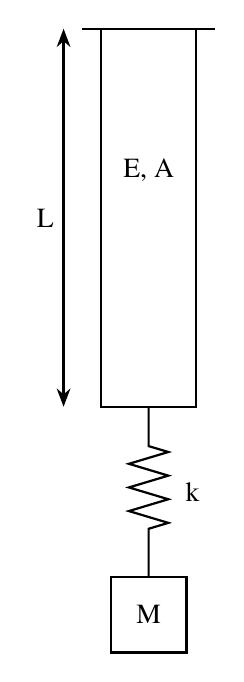
\begin{tikzpicture}[scale=1.2, >=Stealth]
    \draw[thick] (-0.2, 4) -- (1.2, 4);

    \draw[thick] (0, 0) rectangle (1, 4);
    \node at (0.5, 2.5) {E, A};

    \draw[thick, <->] (-0.4, 0) -- (-0.4, 4);
    \node[left] at (-0.4, 2) {L};

    \draw[thick, decorate, decoration={zigzag, segment length=3mm, amplitude=2.5mm, pre length=5mm, post length=5mm}] (0.5, 0) -- (0.5, -1.8);
    \node[right=3pt] at (0.7, -0.9) {k};

    \draw[thick] (0.1, -1.8) rectangle (0.9, -2.6);
    \node at (0.5, -2.2) {M};
\end{tikzpicture}
\end{center}

\subsection*{Step-by-Step Solution:}
\noindent \textbf{Step 1: Axial Stiffness of the Bar ($k_{\text{bar}}$)}\\
The axial stiffness of the uniform bar is:
\begin{align*}
k_{\text{bar}} = \frac{AE}{L}
\end{align*}

\noindent Converting parameters to standard SI units:
\begin{align*}
E &= 200 \times 10^9 \text{ N/m}^2 \\[0.5ex]
A &= 100 \times 10^{-6} \text{ m}^2 = 10^{-4} \text{ m}^2 \\[0.5ex]
L &= 100 \times 10^{-3} \text{ m} = 0.1 \text{ m}
\end{align*}

\begin{align*}
k_{\text{bar}} = \frac{10^{-4} \times 200 \times 10^9}{0.1} = 2 \times 10^8 \text{ N/m}
\end{align*}
\noindent \textbf{Step 2: Equivalent Stiffness ($k_{\text{eq}}$)}\\
The bar and the helical spring are connected in series. Therefore:
\begin{align*}
\frac{1}{k_{\text{eq}}} = \frac{1}{k_{\text{bar}}} + \frac{1}{k}
\end{align*}

\noindent With $k = 200 \text{ kN/mm} = 2 \times 10^8 \text{ N/m}$:
\begin{align*}
k_{\text{eq}} = \frac{k_{\text{bar}} \cdot k}{k_{\text{bar}} + k} = \frac{(2 \times 10^8)(2 \times 10^8)}{2 \times 10^8 + 2 \times 10^8} = 10^8 \text{ N/m}
\end{align*}

\noindent \textbf{Step 3: Natural Frequency ($\omega_n$)}\\
The natural frequency of free vibration is:
\begin{align*}
\omega_n = \sqrt{\frac{k_{\text{eq}}}{M}} = \sqrt{\frac{10^8}{100}} = \sqrt{10^6} = 1000 \text{ rad/s}
\end{align*}

\noindent \textbf{Final Answer:} \textbf{1000}
\newpage

\end{document}
